\section{Results}
In the following sections results will be presented for the AMPL implementation and for both of the heuristics. The parameter values used in the runs will also be presented. 

\subsection{AMPL implementation}

Implementing the model in AMPL and running the model in CPLEX 12.5 gives the resulting values for the three objective function components displayed in Table \ref{tab:CPLEX_res}. The weights in equations \ref{objfcn} and \ref{constr:s_min} were set to $L = 2$, $A = 1$, $M =100$ and $N=1$, thus making librarians twice as valuable as assistants and stand ins 100 times more valuable than no shift changes. 

\begin{table}[!h]
\centering
\label{tab:CPLEX_res}
\caption{Results from running the Mathematical Model in CPLEX.}
\begin{tabular}{|l|p{3cm}|p{3cm}|l|}
\hline
\rowcolor{Gray} & \textbf{Min num stand ins (lib,ass)} & \textbf{Number of shift changes} & \textbf{Solution time} \\ \hline
\cellcolor{Gray} \textbf{Result} & \multicolumn{1}{c|}{(3,0)} & \multicolumn{1}{c|}{0} & \multicolumn{1}{c|}{19 min} \\
\hline
\end{tabular}
\end{table}

These results can be used as benchmark in the heuristics as CPLEX returns an optimal solution. 

\subsection{Weekly scheduling approach}
As most of the costs are correlated with each other some parameter tuning has been required. The final result of the parameter tuning can be seen in Table \ref{tab:cost_parameters}. Their respective descriptions can be seen in Table \ref{tab:all_costs}. 

\begin{table}[!h]
\centering
\caption{List of all costs used in weekly scheduling approach and their respective values.}
\label{tab:cost_parameters}
\begin{tabular}{|l|l|}
\hline
\rowcolor[HTML]{FD6864} 
\multicolumn{2}{|l|}{\cellcolor{corn} \textbf{Demand costs}} \\ \hline
%\multicolumn{2}{|c|}{\cellcolor[HTML]{FD6864}Demand costs}    \\ \hline
\rowcolor[HTML]{C0C0C0} 
Cost name                                      & Value       \\ \hline
Demand\_few\_ass                        & 350         \\ \hline
Demand\_few\_lib                        & 300         \\ \hline
Demand\_many\_ass                       & 200         \\ \hline
Demand\_many\_lib                       & 40          \\ \hline
Demand\_few\_total                             & 800         \\ \hline
Demand\_many\_total                            & 700         \\ \hline
Demand\_evening\_cost         & 20,000 				\\ \hline
Demand\_PL\_good\_ass        & 1,200            \\ \hline
Demand\_PL\_good\_lib        & 800           \\ \hline
Demand\_PL\_bad\_ass         & 1,200           \\ \hline
Demand\_PL\_bad\_lib         & 1,600             \\ \hline
\rowcolor[HTML]{FD6864} 
\multicolumn{2}{|l|}{\cellcolor{corn} \textbf{PL amount costs}} \\ \hline
\rowcolor[HTML]{C0C0C0} 
Cost name                                      & Value       \\ \hline
PL\_good\_amount                  & 1,000                   \\ \hline
PL\_violate\_amount             & 1,500                  \\ \hline
\rowcolor[HTML]{FD6864} 
\multicolumn{2}{|l|}{\cellcolor{corn} \textbf{Weekend costs}} \\ \hline
\rowcolor[HTML]{C0C0C0} 
Cost name                                      & Value       \\ \hline
HB\_amount                       & 15,000    \\ \hline
No\_weekend                & 5,000                   \\ \hline
\rowcolor[HTML]{FD6864} 
\multicolumn{2}{|l|}{\cellcolor{corn} \textbf{Stand-in costs}} \\ \hline
\rowcolor[HTML]{C0C0C0} 
Cost name                                      & Value       \\ \hline
Stand\_in\_cost                     & 5     \\ \hline
\end{tabular}
\end{table}

Worth noting is that these values are most certainly not optimal as they have mostly been assigned using intuition. However, a few relations were determined by either running some tests or using reason. An example is either if $PL\_good\_cost > Demand\_PL\_good\_ass$ or $PL\_good\_cost > Demand\_PL\_good\_lib$. If so, all workers that can be assigned another PL will be, leaving the library overstaffed with PL workers. The reason is because the net of $-PL\_good\_cost + Demand\_PL\_good\_ass/lib$ will be negative meaning it is a preferable insertion even though the library will be overstaffed.

%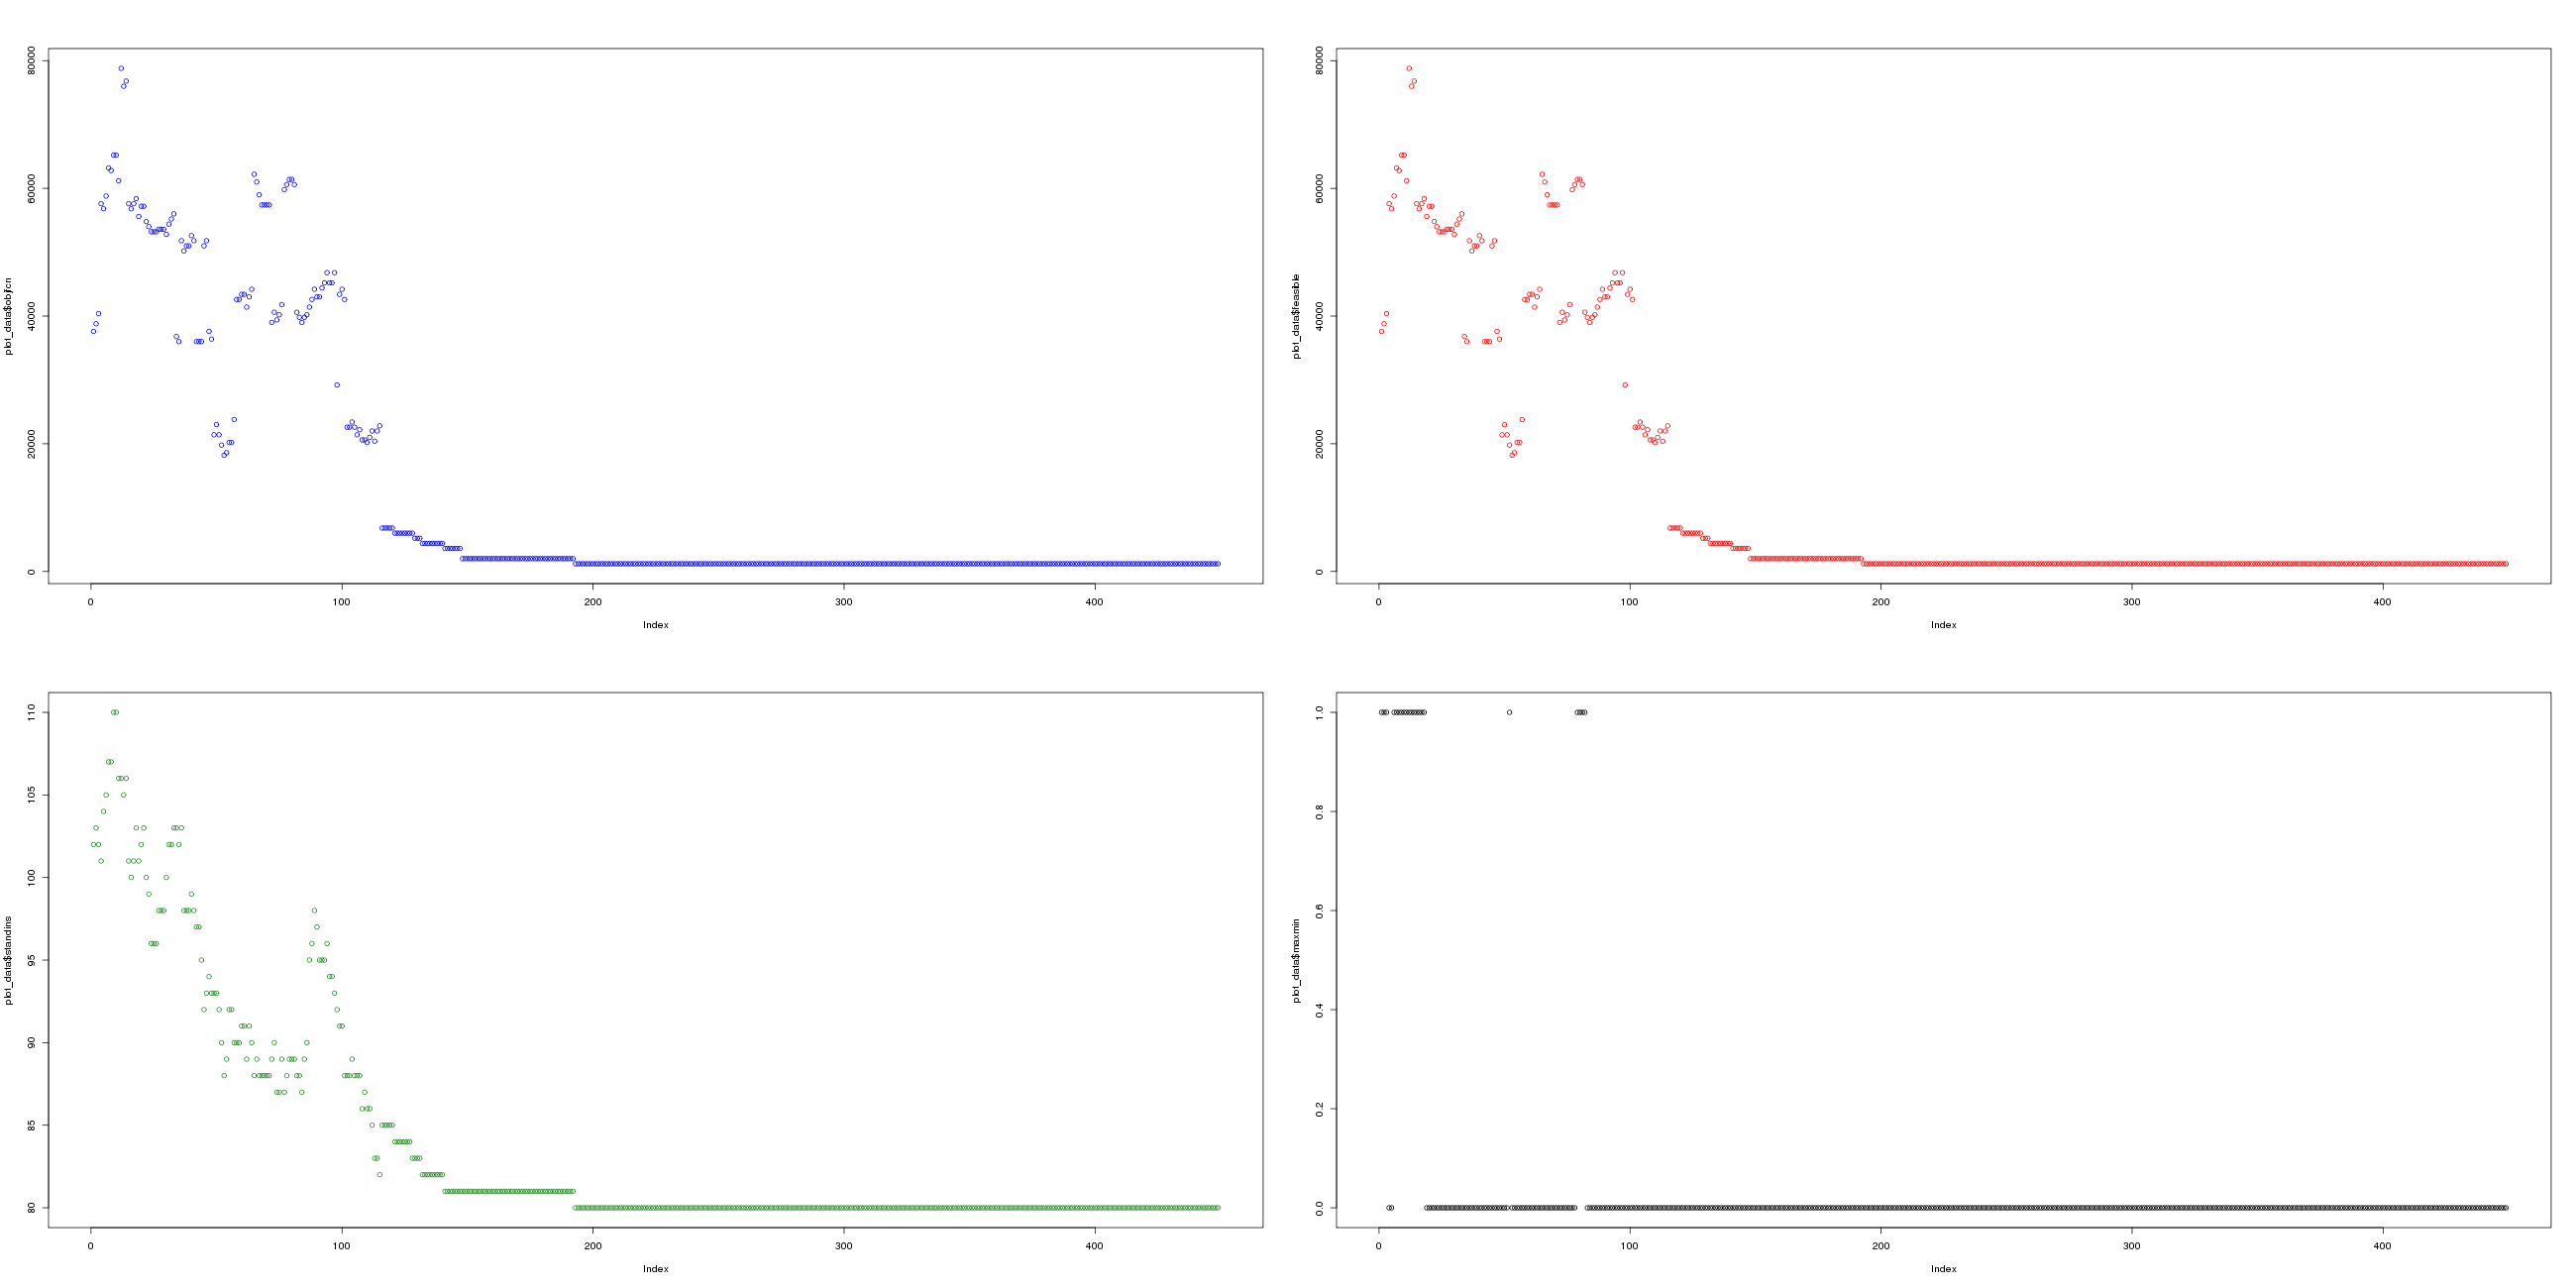
\includegraphics[scale = 0.3, width = 15cm]{Rplot}
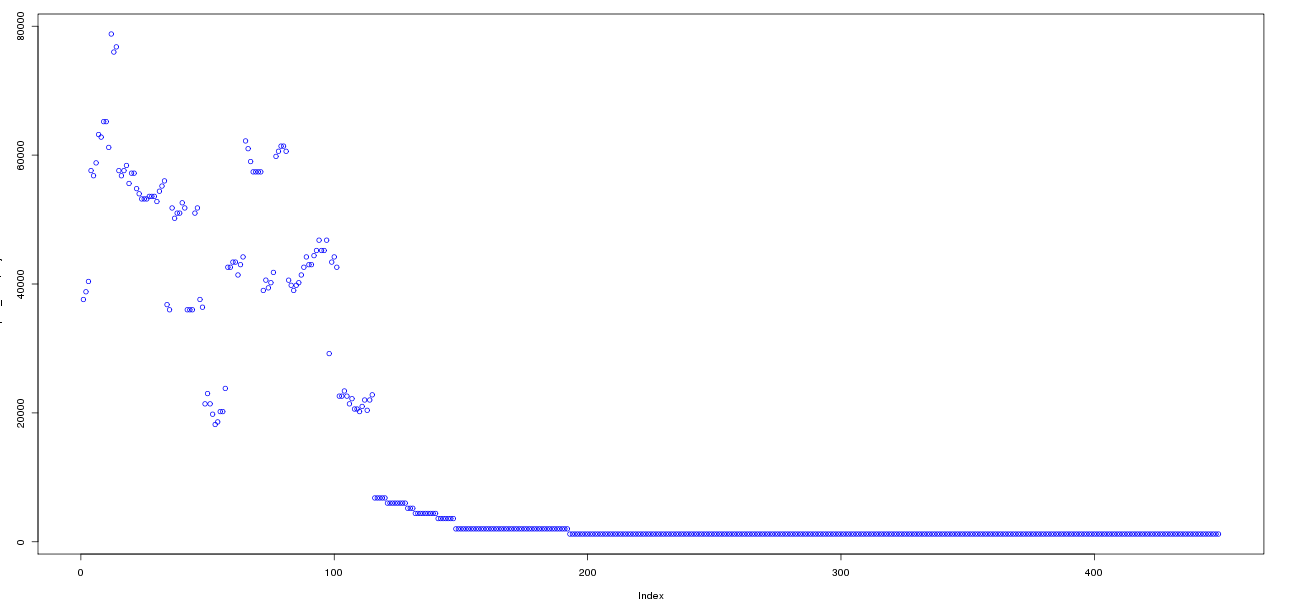
\includegraphics[scale = 0.3, width = 15cm]{1Plot}
\subsection{Task distribution approach}

Some parameter tuning was done in order to find the optimal settings for the algoritm, particularly for the weekend objective function weights described in Section \ref{section:tasks_cost}. The tuning landed in the following parameters
 
Number of iterations, first phase.
Number of iterations, second phase.
$T_0$, $\alpha$


\section{Discussion}
Text


\subsection{Weekly scheduling approach}
Table \ref{pros_cons_weekly_scheduling} lists pros and cons with the implemented weekly scheduling approach. Some pros and cons were considered before the heuristic was chosen. Mainly the con concerning the exponential growth was taken into consideration as an estimation of the upper limit of the problem size was done. Also, the pro regarding the same amount of week blocks was taken into consideration, as the heuristic was thought of having firstly a block construction phase and secondly an assignment phase. 

\begin{table}[!h]
\caption{Pros and cons with the implemented weekly scheduling approach}
\label{pros_cons_weekly_scheduling}
\begin{tabularx}{\linewidth}{>{\parskip1ex}X@{\kern4\tabcolsep}>{\parskip1ex}X}
\toprule
\hfil\bfseries Pros
&
\hfil\bfseries Cons
\\\cmidrule(r{3\tabcolsep}){1-1}\cmidrule(l{-\tabcolsep}){2-2}

%% PROS, seperated by empty line or \par
The same amount of week block appearances will exist for five and ten weeks.\par
Quick iterations when destroying and repairing.\par

&

%% CONS, seperated by empty line or \par
Weekends needs to be assigned in a more systematically way in order to achieve reasonable results regarding lowest amount of stand-ins through the days.\par
The amount of unique block appearances grows exponentially in case more task types are added, such as meetings.\par
The solution time can vary considerably as several random generators have been used.\par
A great deal of costs are needed (some correlated), where each of them affects the solution procedure.

\\\bottomrule
\end{tabularx}
\end{table}

 Weekends, solution time and costs are no major issues as they can be avoided by a few smarter implementations. For instance, weekends can be improved by assigning values when each worker is available on a day and from those numbers create an even distribution of possible stand-ins and therefore increase the lowest value of stand-ins through the days. This shall implicitly decrease the solution time as less iterations will be required. However, to always be able to create a pool of week appearances regardless of problem size can easily become a major issue. Just by adding meetings and the assignment of Library on Wheels tasks to the problem makes it grow considerably.
 

\subsection{Task distribution approach}
Text